
\subsection{Kinect}

El Kinect es un dispositivo desarrollado por Microsoft que consiste en una cámara web junto con un sensor de profundidad. La cámara web es de características relativamente normales, capturando imágenes a una tasa máxima de 30fps y a una resolución de 640 x 480. El dispositivo posee además un acelerómetro para determinar la orientación del mismo respecto del suelo de forma automática.

\image{sensor}{0.5}{Kinect}

El sensor de profundidad captura a la misma frecuencia y resolución que la cámara, y está compuesto por un láser proyector infrarrojo y un sensor CMOS; el primero proyecta continuamente varios haces de luz cuya respuesta al interactuar con el ambiente es medida por el segundo, de manera que se pueda detectar la distancia entre el dispositivo y los objetos de la sala. Esto permite distinguir objetos con mayor facilidad ya que una imagen de profundidad contiene información valiosa para ubicar objetos 3D con una imagen 2D. Esto facilita el proceso de segmentación ya que la imagen de profundidad es una buena aproximación a la profundidad o posición en el eje z de los objetos. Además, al utilizar un láser infrarrojo las condiciones de luz ambiental no afectan tanto este proceso. 

\image{sensor-depth}{0.2}{Imagen capturada con el sensor de profundidad del Kinect}


Acompaña al dispositivo un SDK propietario de detección de personas y las partes de sus cuerpos en tiempo real. Este SDK es desarrollado por la misma compañía que desarrolla el dispositivo, y fue usado en esta tesina sin cambios. A continuación, se describirá el funcionamiento de ambos para que se puedan comprender sus funcionalidades y limitaciones.


El SDK reconoce hasta 4 personas al mismo tiempo y monitorea a una tasa máxima de 30 fps las posiciones de las 20 articulaciones más importantes del cuerpo (solo las de la parte superior del cuerpo en modo sentado) y los ángulos entre ellas en un espacio virtual tridimensional enfrente de la cámara, y relativo a la misma.

\begin{figure}[ht]
\centering
\begin{minipage}[b]{0.3\linewidth}
\centering
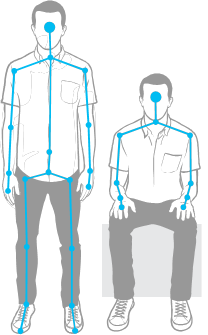
\includegraphics[width=0.5\textwidth]{img/db/skeletons}
\caption{Esqueletos detectados en modo normal y modo sentado}
\label{fig:esqueletos}
\end{minipage}
\hspace{0.5cm}
\begin{minipage}[b]{0.40\linewidth}
\centering
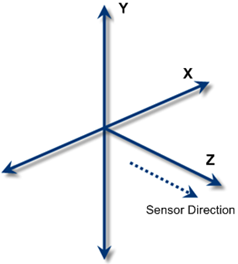
\includegraphics[width=0.5\textwidth]{img/db/sensor-axes}
\caption{Ejes del kinect. El centro de coordenadas corresponde a la posición de la cámara}
\label{fig:ejeskinect}
\end{minipage}
\end{figure}



Para un correcto funcionamiento del reconocimiento, el usuario debe posicionarse a una distancia de la cámara de entre 0.8m y 4m en el modo normal, y entre 0.4m y 3m en el modo de cercanía. 

\image{sensor-range}{0.5}{Rango del sensor}

El ángulo de visión horizontal es de 57 grados y el vertical de 43 grados. Cuando la cámara  funciona en el modo normal, a la distancia mínima de 0.8m, la cámara captura 87cm de forma horizontal (eje x) y 66 cm de forma vertical (eje y); a medida que la distancia a la cámara crece, aumenta también el área de captura.


\subsection{SDK y Algoritmo de tracking del cuerpo}

El reconocimiento del SDK del Kinect está orientado a movimientos «gruesos»; por ejemplo, detecta los movimientos de la mano, no de los dedos. Puede distinguir distintas personas y sus movimientos, aun cuando estén parcialmente ocultos, ya que extrapola la posición de las partes del cuerpo ocultas a partir de las visibles. 

El núcleo del algoritmo de reconocimiento del Kinect trabaja sobre imágenes individuales tomadas por el sensor de profundidad, que son segmentadas etiquetando partes del cuerpo de forma probabilística; las partes del cuerpo a etiquetar son aquellas que se encuentren espacialmente cerca de las articulaciones que se quieren reconocer. Reproyectando las partes inferidas en el espacio 3D virtual, se localizan los modos espaciales de la distribución de probabilidad de cada parte del cuerpo, y así se generan varias propuestas para las ubicaciones en 3D  de cada una de las articulaciones del cuerpo, cada una con cierto puntaje de confianza. La segmentación en partes del cuerpo se realiza como una clasificación por pixel para evitar la explosión combinatoria que implicaría una búsqueda sobre las distintas propuestas de posiciones de articulaciones del cuerpo; esta debilidad del método se balancea con la gran cantidad de imágenes de profundidad de entrenamiento utilizadas. 

Para lograr esto, los autores del SDK en una primera etapa crearon una base de datos con imágenes de profundidad reales de personas realizando distintos movimientos en condiciones ambientales muy diferentes, en las cuales las partes del cuerpo se etiquetaron a mano. En base a eso, generaron un modelo de movimiento humano en 3 dimensiones, mediante el cual luego generaron una cantidad enorme de datos sintéticos, con imágenes de profundidad sintéticas de humanos de distintas formas y tamaños en poses muy variadas. Entrenaron un conjunto de árboles de decisión aleatorizados (\textbf{Random Forest}) \cite{breiman2001random} que evita el sobreentrenamiento y obtiene invariancia a la traslación 3D gracias a esta gigantesca cantidad de datos. Finalmente, utilizando el algoritmo \textbf{mean-shift} \cite{comaniciu2002mean}, se infieren los modos espaciales de las distribuciones por pixel de las cuales se extraen distintas propuestas de las posiciones 3D de las articulaciones. 

En todo este proceso, no se utiliza ninguna información temporal, ni datos extraídos de imágenes anteriores, lo cual lo hace más robusto y permite una re-inicialización rápida cuando una persona sale y entra al campo de visión de la cámara, o es temporalmente obstruida por otra persona u objeto \cite{Shotton2011}.  


\image{sensor-recognition-process}{0.3}{ Imagen de profundidad $\rightarrow$  Partes del cuerpo $\rightarrow$ Modelos 3D propuestos}

El SDK se puede utilizar con un mecanismo de polling o mediante callbacks que se realizan a la tasa máxima de 30fps mencionada anteriormente. En ambos casos, en cada poll o callback la información que se provee es la cantidad de esqueletos (personas) detectados, con un identificador que se mantiene en el tiempo, y para cada uno la posición de 20 articulaciones del cuerpo, donde para cada una se indica si esta posición ha sido detectada normalmente, ha sido inferida a través de las posiciones de otras articulaciones, o si no ha sido posible detectarla. Adicionalmente, para cada esqueleto se estima la ecuación $Ax+By+Cz+D=0$ que describe el plano definido implícitamente por el suelo respecto a la cámara, normalizada de manera tal que $D$ representa la distancia entre el suelo y la cámara.
